\begin{figure}[htbp]
\centering
\vspace{-2mm}
 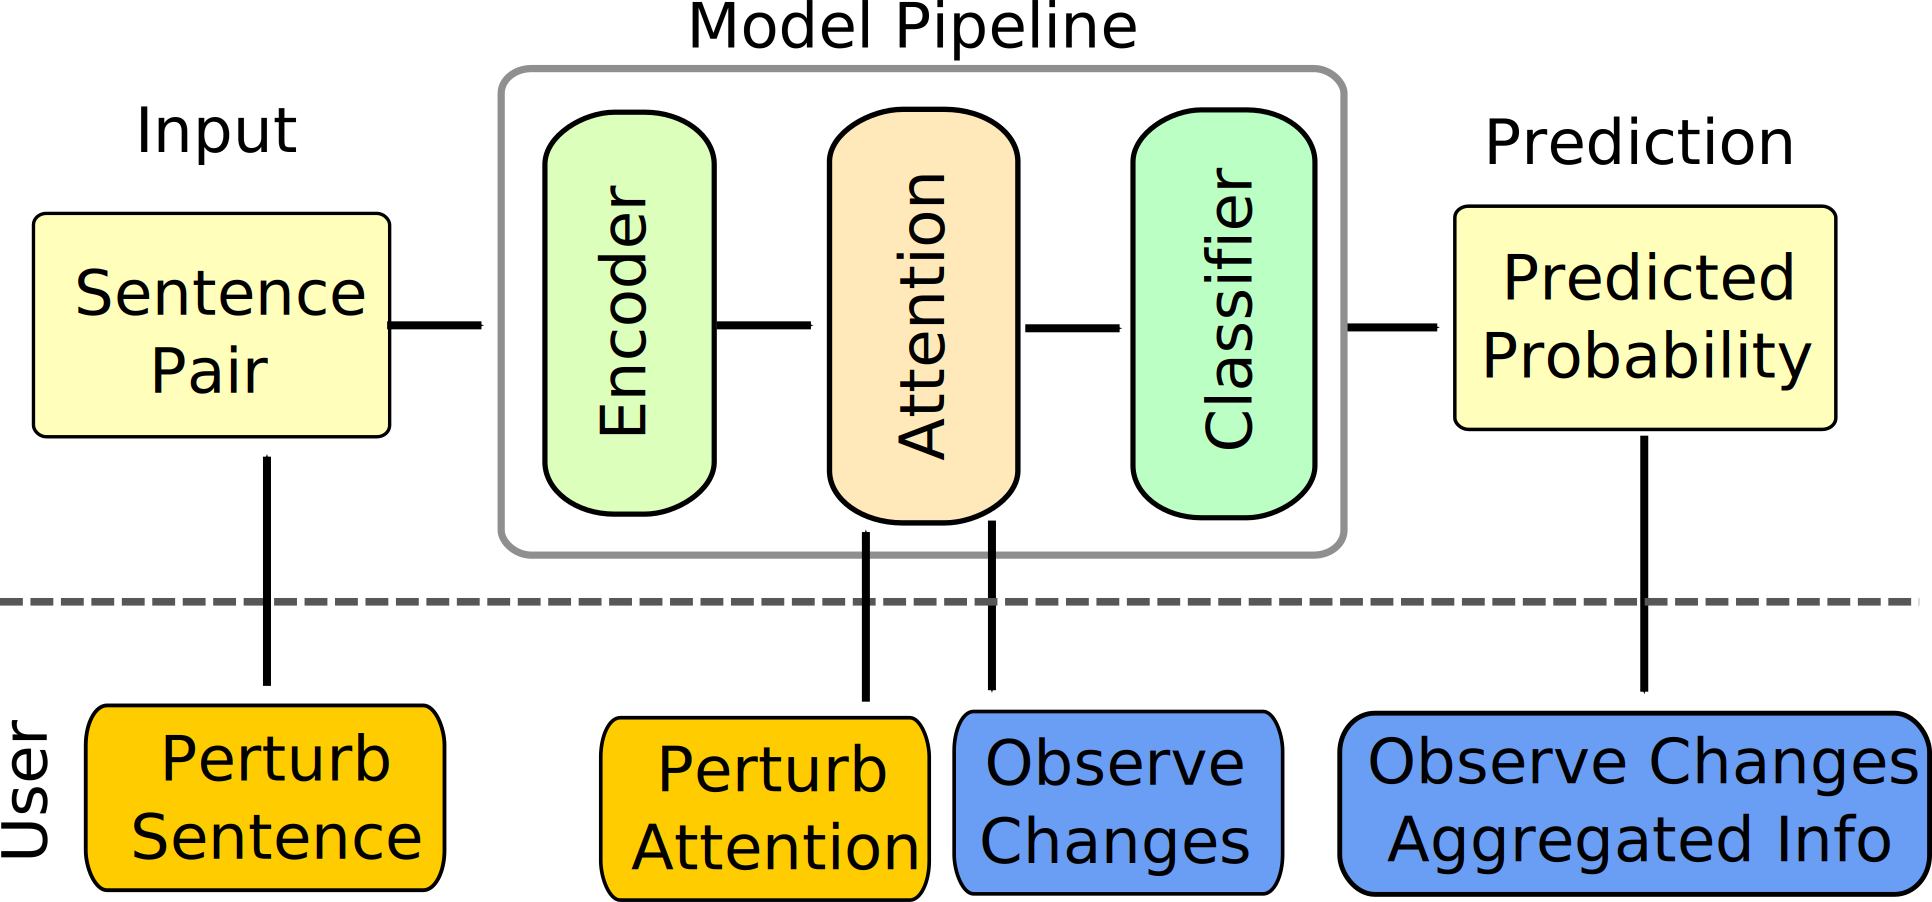
\includegraphics[width=1.0\linewidth]{pipeline}
 \caption{
 Perturbation-Driven Exploration of the Language Inference Model.
 }
\label{fig:modelPipeline}
\end{figure}

\subsection{Perturbation-Driven Exploration}

Fig.~\ref{fig:modelPipeline}

Understand where and how does a model fail is the first step to improve the
model performance.
Prediction accuracy, i.e., the percentage of the correct prediction according to
the ground truth label, is the standard technique to verify the performance
of a model on a given supervised task.
%
The accuracy alone does not tell us the whole story, it provides no
information on the specific example and the condition that lead to a failure.
%
Often, the user need to examine individual failure examples to diagnostic the
issue and identify the weakness of the model.
%
However, the model may be unstable and generate the right prediction for the wrong
reason (e.g., by picking up noise in the data that is not the intended features),
therefore, we are likely to miss some important failure condition by just looking
at the failure cases.
%
An in depth analysis of the error made by the model requires the verification of
the robustness of the prediction.
%
One powerful tool to assess robustness is through the application of small
perturbation in the input and then check the variation of the prediction.
%
For example, we can replace noun and verb in the sentences with words of
similar/same meaning, such an operation is often carried out by domain experts
(subconsciously) when they try to figure out the potential issue of a model.
%
In another work, the perturbation of the input allow us to do a sensitivity
analysis on the prediction.
%
In this work, we introduce an synonyms perturbation scheme that automatically
generate the perturbation and generate the prediction and summarized the prediction
variation.
%


% \begin{itemize}
%     \item perturbation prediction change ratio
%     \item distribution distance (KL divergence) to original prediction
%     \item attention change distance
% \end{itemize}

%%%%%%%% Overview figure for the pipeline %%%%%%%%%%
% \begin{figure}
%     \includegraphics{/path/to/figure}
%     \caption{}
%     \label{}
% \end{figure}

% \subsection{Input Perturbation}

Iterate the model design and debug the system hinged on the ability to quickly and identify the errors made by a model.

Perturbation the input is what NLP researchers have subconsciously been doing to study and test a model.

Interpret/probe the relationship between attention and the prediction result


% \subsection{Attention Perturbation}


% \subsection{Prediction Perturbation}
